\documentclass{beamer}

%\includeonlyframes{current}

\usepackage[T1]{fontenc}
\usepackage[utf8]{inputenc}
\usepackage[american]{babel}
\usepackage{amsmath,amssymb,amsthm}
\usepackage{tikz}
\usepackage[backend=biber,citestyle=authoryear-comp,bibstyle=beamer,doi=false,isbn=false,url=false,maxnames=10]{biblatex}
\bibliography{defeo}

\mode<presentation>{%
  \usetheme{Boadilla}
}
\beamertemplatenavigationsymbolsempty

\usepackage{sourcesanspro}
\usepackage[amssymb,amsfonts]{concmath}
\usefonttheme[onlymath]{serif}

\renewcommand{\emph}[1]{{\usebeamercolor[fg]{structure}#1}}

%\let\footcite\footnote

\newcommand{\C}{\mathbb{C}}
\newcommand{\R}{\mathbb{R}}
\newcommand{\Z}{\mathbb{Z}}
\newcommand{\N}{\mathbb{N}}
\newcommand{\Q}{\mathbb{Q}}
\newcommand{\F}{\mathbb{F}}
\renewcommand{\P}{\mathbb{P}}
\renewcommand{\O}{\mathcal{O}}
\newcommand{\tildO}{\mathcal{\tilde{O}}}
\newcommand{\End}{\operatorname{End}}
\newcommand{\chr}{\operatorname{char}}
\newcommand{\Cl}{\operatorname{Cl}}
\renewcommand{\a}{{\mathfrak{a}}}
\renewcommand{\b}{{\mathfrak{b}}}
\newcommand{\cyc}[1]{{\langle #1 \rangle}}
\newcommand{\ord}{\operatorname{ord}}

\usetikzlibrary{arrows,matrix,decorations,decorations.text,decorations.pathmorphing,calc}

\pgfkeys{/triangle/.code=\tikzset{x={(-0.5cm,-0.866cm)},y={(1cm,0cm)}}}
\pgfkeys{/lattice/.code n args={4}{\tikzset{cm={#1,#2,#3,#4,(0,0)}}}}

\newcommand{\axes}[4]{
  \clip (#1,#3) rectangle (#2,#4);
  \draw [thin, gray, -latex] (#1,0) -- (#2,0);% Draw x axis
  \draw [thin, gray, -latex] (0,#3) -- (0,#4);% Draw y axis
}

\newcommand{\lattice}[2]{
  \draw[style=help lines,dashed] (#1-1,#1-1) grid[step=1] (#2+1,#2+1);
  \foreach \x in {#1,...,#2}{
    \foreach \y in {#1,...,#2}{
      \node[draw,circle,inner sep=2pt,fill] at (\x,\y) {};
      % Places a dot at those points
    }
  }
}

\newcommand{\bl}[1]{\textcolor{blue}{#1}}
\newcommand{\rd}[1]{\textcolor{red}{#1}}
\newcommand{\gr}[1]{\textcolor{green}{#1}}

% This command defines a triangle of dots of given height
\newcommand{\dottriangle}[2][\i-\j]{%
  \foreach \i in {0,...,#2} {%
    \foreach \j in {0,...,\i} {%
      \draw(\i,\j) node{#1};%
    }%
  }}


\title{Isogeny graphs in cryptography}
\author[Luca De Feo]{Luca De Feo}
\date[Mar 19--23, 2018 --- Post-Scryptum]{March 19--23, 2018, Post-Scryptum Spring School,
  Les 7 Laux
}
\institute[U Paris Saclay]{Université Paris Saclay, UVSQ \& Inria}

\begin{document}

\frame[plain]{
  \begin{tikzpicture}[remember picture,overlay]
    \node[at=(current page.center), opacity=0.7] {
      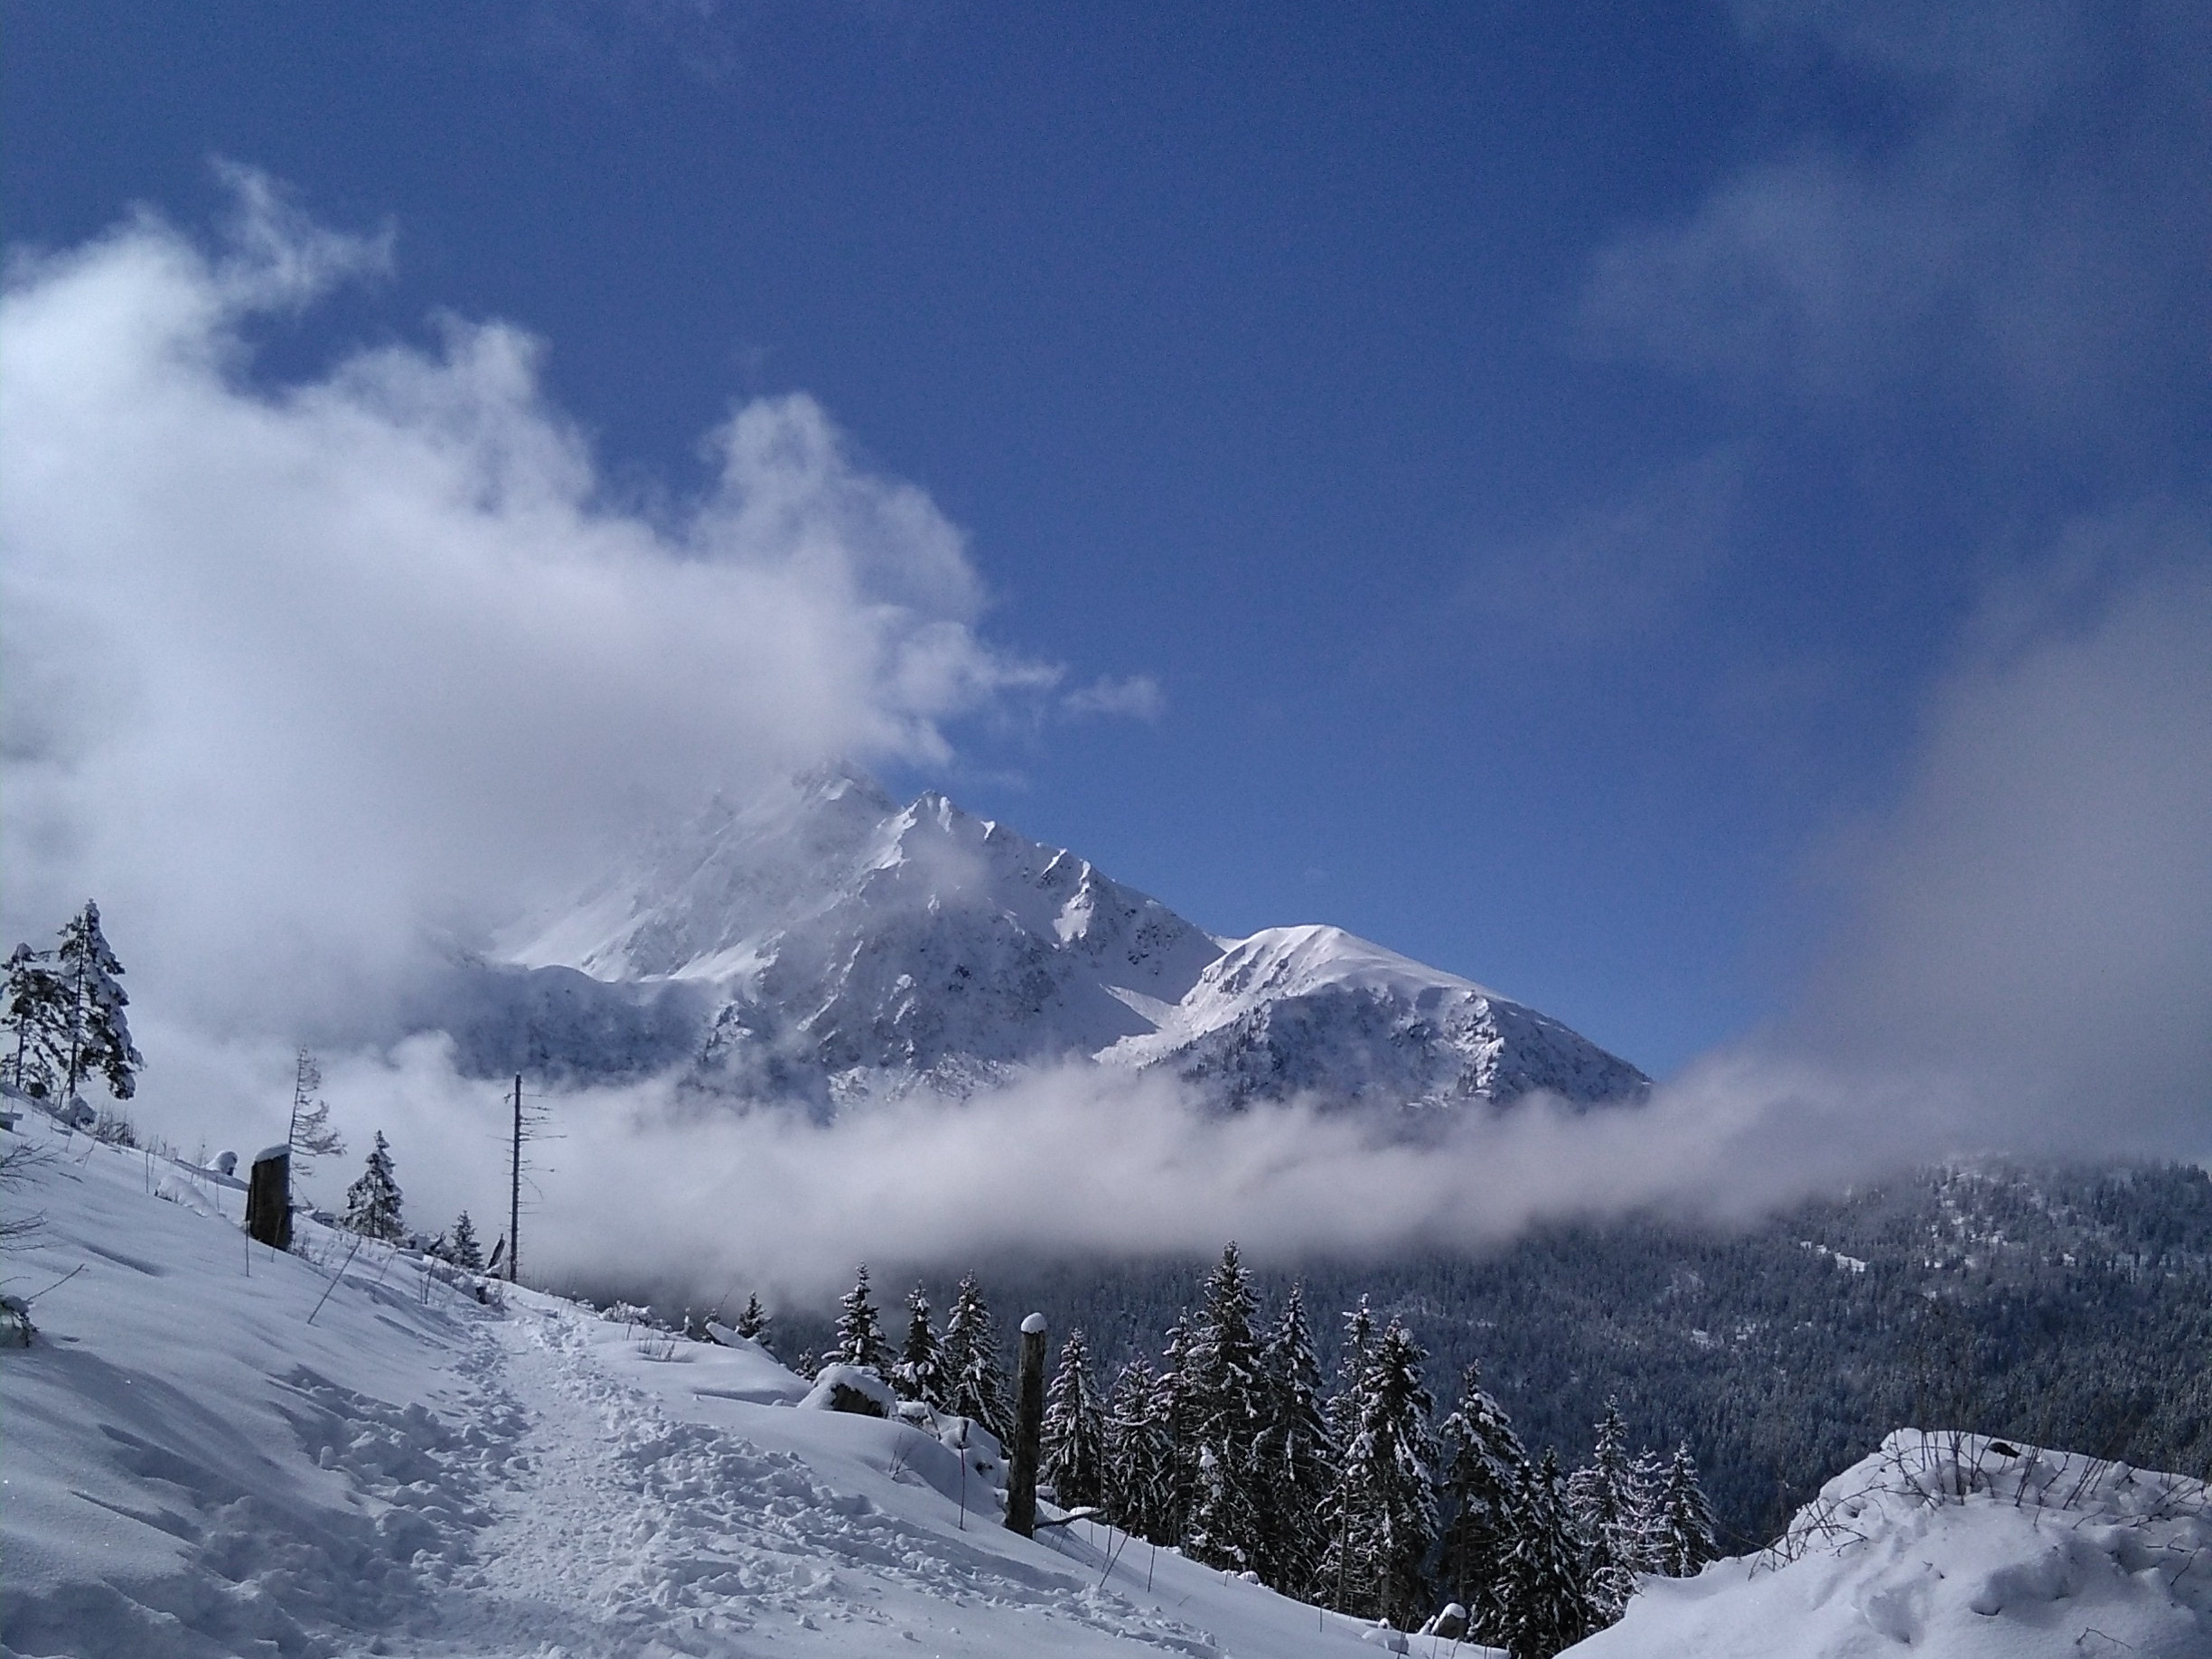
\includegraphics[width=1.2\paperwidth]{7laux.jpg}
    };
    \node[yshift=1em,xshift=5em,at=(current page.south west)]{\tiny Photo courtesy of Elisa Lorenzo-García};
  \end{tikzpicture}
  \vspace{-1.1cm}
  {\bf \titlepage}
  \vspace{0.5cm}
  \begin{center}
    Slides online at~~~\emph{\url{http://defeo.lu/docet/}}
  \end{center}
}

%% 

\begin{frame}
  \frametitle{Overview}
  \tableofcontents  
\end{frame}

%%
%% 

\section{Foundations}

\subsection{Elliptic curves}

\begin{frame}{Projective space}
  \begin{definition}[Projective space]
    Let $\bar{k}$ an algebraically closed field, the \emph{projective
      space} $\P^n(\bar{k})$ is the set of non-null $(n+1)$-tuples
    $(x_0,\dots,x_n)\in \bar{k}^n$ modulo the equivalence relation
    \[(x_0,\dots,x_n) \sim (\lambda x_0, \dots, \lambda x_n) \qquad
      \text{with $\lambda\in \bar{k}\setminus\{0\}$}.\]
    A class is denoted by $(x_0:\cdots:x_n)$.
  \end{definition}

  Picture here
\end{frame}

%%

\begin{frame}{Weierstrass equations}
  \begin{columns}
    \begin{column}{0.4\textwidth}
      Let $k$ be a field of characteristic $\ne 2,3$.

      An \emph{elliptic curve \textit{defined over $k$}} is the locus
      in $\P^2(\bar{k})$ of an equation
      \[\emph{Y^2Z = X^3 + aXZ^2 + bZ^3},\]
      where $a,b\in k$ and $4a^3+27b^2\ne 0$.

      \begin{itemize}
      \item<2-> $\O=(0:1:0)$ is the \emph{point at infinity};
      \item<3-> $y^2 = x^3 + ax + b$ is the \emph{affine equation}.
      \end{itemize}
    \end{column}
    \begin{column}{0.6\textwidth}
      \begin{center}
        \begin{tikzpicture}[domain=-2.4566:4,samples=100,yscale=1/2]
          \draw plot (\x,{sqrt(\x*\x*\x-4*\x+5)});
          \draw plot (\x,{-sqrt(\x*\x*\x-4*\x+5)});

          \draw[thin,gray,-latex] (0,-7) -- (0,7);
          \draw[thin,gray,-latex] (-3,0) -- (4,0);
        \end{tikzpicture}
      \end{center}
    \end{column}
  \end{columns}
\end{frame}

%%

\begin{frame}{The group law}
  \begin{columns}
    \begin{column}{0.4\textwidth}
      \begin{block}{Bezout's theorem}
        Every line cuts $E$ in exactly three points (counted with
        multiplicity).
      \end{block}

      Define a \emph{group law} such that any three colinear points
      add up to zero.

      \begin{itemize}
      \item<2-> The law is \emph{algebraic}\\ (it has \textit{formulas});
      \item<3-> The law is \emph{commutative};
      \item<3-> $\O$ is the \emph{group identity};
      \item<3-> \emph{Opposite points} have the same $x$-value.
      \end{itemize}
    \end{column}
    \begin{column}{0.6\textwidth}
      \begin{center}
        \begin{tikzpicture}[domain=-2.4566:4,samples=100,yscale=1/2]
          \draw plot (\x,{sqrt(\x*\x*\x-4*\x+5)});
          \draw plot (\x,{-sqrt(\x*\x*\x-4*\x+5)});

          \draw[thin,gray,-latex] (0,-7) -- (0,7);
          \draw[thin,gray,-latex] (-3,0) -- (4,0);
          \draw (-3,1) -- (4,8/3+3);
          \begin{scope}[every node/.style={draw,circle,inner sep=1pt,fill},cm={1,2/3,0,0,(0,3)}]
            \node at (-2.287980,0) {};
            \node at (-0.535051,0) {};
            \node at (3.267475,0) {};
          \end{scope}
          \begin{scope}[every node/.style={yshift=0.3cm},cm={1,2/3,0,0,(0,3)}]
            \node at (-2.287980,0) {$P$};
            \node at (-0.535051,0) {$Q$};
            \node at (3.267475,0) {$R$};
          \end{scope}

          \draw[dashed] (3.267475,3.267475*2/3+3) -- (3.267475,-3.267475*2/3-3) 
          node[draw,circle,inner sep=1pt,fill] {}
          node[xshift=-0.1cm,anchor=east] {$P+Q$};
        \end{tikzpicture}
      \end{center}
    \end{column}
  \end{columns}
\end{frame}

%%

\begin{frame}{Group structure}
  \begin{block}{Torsion structure}
    Let $E$ be defined over an algebraically closed field $\bar{k}$ of
    characteristic $p$.
    \begin{align*}
      E[m] \simeq\quad& \Z/m\Z\times\Z/m\Z  &\text{if $p\nmid m$,}\\[1em]
                 &\Z/p^e\Z & \text{\emph{ordinary} case,}\\[-1.7em]
      E[p^e] \simeq\Biggl\{& \\[-1.7em]
%               \begin{cases}
                 &\{\O\} & \text{\emph{supersingular} case.}
%               \end{cases}
    \end{align*}
  \end{block}

  \begin{block}{Free part}
    Let $E$ be defined over a \emph{number field} $k$, the group of
    $k$-rational points $E(k)$ is \emph{finitely generated}.
  \end{block}
\end{frame}

%%

\begin{frame}{Maps: isomorphisms}
  \begin{block}{Isomorphisms}
    The only \emph{invertible algebraic maps} between elliptic curves
    are of the form
    \[(x,y) \mapsto (u^2x, u^3y)\]
    for some $u\in\bar{k}$.

    They are \emph{group isomorphisms}.
  \end{block}

  \begin{block}{$j$-Invariant}
    Let $E\;:\;y^2=x^3+ax+b$, its \emph{$j$-invariant} is
    \[j(E) = 1728\frac{4a^3}{4a^3+27b^2}.\]

    Two elliptic curves $E,E'$ are \emph{isomorphic} if and only if
    $j(E)=j(E')$.
  \end{block}
\end{frame}

%%

\begin{frame}{Maps: isogenies}
  \begin{theorem}
    Let $\phi:E\to E'$ be a map between elliptic curves. These
    conditions are equivalent:
    \begin{itemize}
    \item $\phi$ is a \emph{surjective group morphism},
    \item $\phi$ is a \emph{group morphism} with \emph{finite kernel},
    \item $\phi$ is a non-constant \emph{algebraic map} of projective
      varieties sending the point at infinity of $E$ onto the point at
      infinity of $E'$.
    \end{itemize}
    If they hold $\phi$ is called an \emph{isogeny}.
  \end{theorem}

  Two curves are called \emph{isogenous} if there exists an isogeny
  between them.

  \begin{block}{Example: Multiplication-by-$m$}
    On any curve, an isogeny from $E$ to itself (i.e., an
    \emph{endomorphism}):
    \begin{align*}
      [m] \;:\; E &\to E,\\
      P &\mapsto [m]P.
    \end{align*}
  \end{block}
\end{frame}

%%

\begin{frame}{Isogenies: an example over $\F_{11}$}
  \begin{tikzpicture}[scale=0.4]
    \begin{scope}
      \node[anchor=center] at (0,7) {$E \;:\; y^2 = x^3 + x$};

      \uncover<-1>{
        \draw[thin,gray] (0,-6) -- (0,6);
        \draw[thin,gray] (-6,0) -- (6,0);
      }

      \foreach \x/\y in {0/0,5/3,-4/3,-3/5,-2/1,-1/3} {
        \draw[blue,fill] (\x,\y) circle (0.2) node(E_\x_\y){}
        (\x,-\y) circle (0.2) node(E_\x_-\y){};
      }

      \uncover<4->{\draw[red,fill] (0,0) circle (0.3);}
    \end{scope}

    \draw[black!10!white,thick] (8,-7) -- +(0,14);
    
    \begin{scope}[shift={(16,0)}]
      \node at (0,7) {$E' \;:\; y^2 = x^3 - 4x$};

      \uncover<-1>{
        \draw[thin,gray] (0,-6) -- (0,6);
        \draw[thin,gray] (-6,0) -- (6,0);
      }

      \foreach \x/\y in {0/0,2/0,3/2,4/2,6/4,-2/0,-1/5} {
        \draw[color=blue,fill] (\x,\y) circle (0.2) node(F_\x_\y){}
        (\x,-\y) circle (0.2) node(F_\x_-\y){};
      }
    \end{scope}

    \begin{scope}[color=red,-latex,dashed]
      \begin{uncoverenv}<2->
        \path
        (E_5_3) edge (F_3_2)
        (E_-4_3) edge (F_4_-2)
        (E_-3_5) edge (F_4_2)
        (E_-2_1) edge (F_3_-2)
        (E_-1_3) edge (F_-2_0);
      \end{uncoverenv}
      \begin{uncoverenv}<2,5->
        \path
        (E_5_-3) edge (F_3_-2)
        (E_-4_-3) edge (F_4_2)
        (E_-3_-5) edge (F_4_-2)
        (E_-2_-1) edge (F_3_2)
        (E_-1_-3) edge (F_-2_0);
      \end{uncoverenv}
    \end{scope}
  \end{tikzpicture}
  
  \begin{columns}
    \begin{column}{0.5\textwidth}
      \[\phi(x,y) = \left(\frac{x^2 + 1}{x},\quad y\frac{x^2-1}{x^2}\right)\]
    \end{column}
    \begin{column}{0.5\textwidth}
      \begin{itemize}
      \item<4-> Kernel generator in \alert{red}.
      \item<5-> This is a degree $2$ map.
      \item<6-> Analogous to $x\mapsto x^2$ in $\F_q^*$.
      \end{itemize}
    \end{column}
  \end{columns}
\end{frame}

%%

\begin{frame}{Curves over finite fields}
  \begin{block}{Frobenius endomorphism}
    Let $E$ be defined over $\F_q$. The \emph{Frobenius endomorphism}
    of $E$ is the map
    \[\pi \;:\; (X:Y:Z) \mapsto (X^q:Y^q:Z^q).\]
  \end{block}

  \begin{block}{Hasse's theorem}
    Let $E$ be defined over $\F_q$, then
    \[\lvert\#E(k)-q-1\rvert\le 2\sqrt{q}.\]
  \end{block}

  \begin{block}{Serre-Tate theorem}
    Two elliptic curves $E,E'$ defined over a finite field $k$ are
    \emph{isogenous over $k$} if and only if $\#E(k)=\#E'(k)$.
  \end{block}
\end{frame}

%%
%% 

\subsection{Isogenies}

\begin{frame}{Complex tori}
  \begin{columns}
    \begin{column}{0.75\textwidth}
      \begin{tikzpicture}[scale=2]
        \axes{-1}{3.5}{-0.5}{3}

        \begin{scope}[/lattice={1}{0.2}{0.4}{0.7}]
          \begin{uncoverenv}<1>
            \draw[fill,black!10] (0,0) -- (1,0) -- (1,1) -- (0,1) -- (0,0);
            \node at (0.5,0.5) {$\C/\Lambda$};
            \node at (0.9,-0.1) {$\omega_1$};
            \node at (-0.1,0.9) {$\omega_2$};
          \end{uncoverenv}

          \lattice{-3}{4}

          \begin{uncoverenv}<2-5>
            \node[red] at (0.7,0.65) {$a$}; 
            \node[draw,circle,inner sep=1pt,fill,red] at (0.8,0.5) {};
            \node[red] at (0.2,0.9) {$b$}; 
            \node[draw,circle,inner sep=1pt,fill,red] at (0.3,0.7) {};
            
            \begin{uncoverenv}<3-4>
              \node[red] at (1.2,1.3) {$a+b$}; 
              \node[draw,circle,inner sep=1pt,fill,red] at (1.1,1.2) {};
              \begin{uncoverenv}<3>
                \draw[red,thin] (0,0) -- (0.8,0.5) -- (1.1,1.2);
                \draw[red,thin] (0,0) -- (0.3,0.7) -- (1.1,1.2);          
              \end{uncoverenv}
            \end{uncoverenv}

            \transdissolve<5>
            \begin{uncoverenv}<5>
              \node[red] at (0.2,0.3) {$a+b$}; 
              \node[draw,circle,inner sep=1pt,fill,red] at (0.1,0.2) {};
            \end{uncoverenv}
          \end{uncoverenv}
        \end{scope}  
      \end{tikzpicture}
    \end{column}
    \begin{column}{0.2\textwidth}
      \begin{onlyenv}<1>
        Let $\omega_1,\omega_2\in\C$ be linearly independent complex
        numbers. Set
        \[\emph{\Lambda = \omega_1\Z \oplus \omega_2\Z}\]

        $\C/\Lambda$ is a \emph{complex torus}.
      \end{onlyenv}

      \begin{onlyenv}<2->
        Addition law induced by addition on $\mathbb{C}$.
      \end{onlyenv}
    \end{column}
  \end{columns}
\end{frame}

%%

\begin{frame}{Homotheties}
  \begin{columns}
    \begin{column}{0.7\textwidth}
      \begin{tikzpicture}[scale=2]
        \axes{-1}{3.3}{-0.5}{3}

        \newcount\scale
        \animate<1-21>
        \animatevalue<1-21>{\scale}{0}{20}
        \begin{uncoverenv}<1-22>
          \begin{scope}[/lattice={1}{0.2}{0.4}{0.7},scale=1+\the\scale/20,rotate=\the\scale]
            \lattice{-3}{4}
            \node[red,yshift=0.2cm] at (0.8,0.5) {$a$}; 
            \node[draw,circle,inner sep=1pt,fill,red] at (0.8,0.5) {};
          \end{scope}
        \end{uncoverenv}
      \end{tikzpicture}      
    \end{column}
    \begin{column}{0.25\textwidth}
      Two lattices are \emph{homotetic} if there exist $\alpha\in\C$
      such that
      \[\emph{\alpha\Lambda_1 = \Lambda_2}\]
    \end{column}
  \end{columns}
\end{frame}  

%%

\begin{frame}{The $j$-invariant}
  We want to classify complex lattices/tori \emph{up to homothety}.

  \begin{block}{Eisenstein series}
    Let $\Lambda$ be a complex lattice. For any integer $k>0$ define
    \[G_{2k}(\Lambda)=\sum_{\omega\in\Lambda\setminus\{0\}}\omega^{-2k}.\]
    Also set
    \[g_2(\Lambda) = 60G_4(\Lambda),\qquad
      g_3(\Lambda) = 140G_6(\Lambda).\]
  \end{block}

  \begin{block}{Modular $j$-invariant}
    Let $\Lambda$ be a complex lattice, the \emph{modular
      $j$-invariant} is
    \[j(\Lambda) = 1728\frac{g_2(\Lambda)^3}{g_2(\Lambda)^3 - 27g_3(\Lambda)^2}.\]
    Two lattices $\Lambda,\Lambda'$ are
    homothetic if and only if $j(\Lambda)=j(\Lambda')$.
  \end{block}
\end{frame}

%%

\begin{frame}{Elliptic curves over $\C$}
  \begin{block}{Weierstrass $\wp$ function}
    Let $\Lambda$ be a complex lattice, the \emph{Weierstrass $\wp$
      function} associated to $\Lambda$ is the series
    \[\wp(z;\Lambda) = \frac{1}{z^2}
      + \sum_{\omega\in\Lambda\setminus\{0\}} \left(\frac{1}{(z-\omega)^2} - \frac{1}{\omega^2}\right).\]
  \end{block}

  Fix a lattice $\Lambda$, then $\wp$ and its derivative $\wp'$ are
  \emph{elliptic functions}:
  \[\wp(z+\omega) = \wp(z),\qquad\wp'(z+\omega) = \wp'(z)\]
  for all $\omega\in\Lambda$.
\end{frame}

\begin{frame}{Uniformization theorem}
  Let $\Lambda$ be a complex lattice. The curve
  \[E\;:\;y^2=\emph{4}x^3 \emph{- g_2(\Lambda)}x \emph{- g_3(\Lambda)}\]
  is an elliptic curve over $\C$. The map
  \begin{align*}
    \C/\Lambda &\to E(\C),\\
    0 &\mapsto (0:1:0),\\
    z &\mapsto (\wp(z):\wp'(z):1)
  \end{align*}
  is an \emph{isomorphism of Riemann surfaces} and a \emph{group morphism}.

  \smallskip
  
  Conversely, for any elliptic curve
  \[E \;:\; y^2 = x^3 + ax + b\]
  there is a unique complex lattice $\Lambda$ such that
  \[g_2(\Lambda) = -4a,\qquad g_3(\Lambda) = -4b.\]
  Moreover \emph{$j(\Lambda) = j(E)$}.
\end{frame}

%%

\begin{frame}
  \frametitle{Multiplication}

  \begin{tikzpicture}[scale=2.2]
    \axes{-1}{4.5}{-0.5}{3}

    \begin{scope}[/lattice={1}{0.2}{0.4}{0.7}]
      \lattice{-3}{5}
    
      \node[red,yshift=0.2cm] at (0.8,0.6) {$a$}; 
      \draw[red] (0.8,0.6) node[fill,circle,inner sep=1pt] {};

      \begin{uncoverenv}<2>
        \node[red,yshift=0.2cm] at (2.4,1.8) {$[3]a$}; 
        \draw[red] (0,0) -- (1.6,1.2) node[fill,circle,inner sep=1pt] {} 
        -- (2.4,1.8) node[fill,circle,inner sep=1pt] {};
      \end{uncoverenv}

      \transdissolve<3>
      \begin{uncoverenv}<3>
        \node[red,yshift=0.3cm] at (0.4,0.8) {$[3]a$}; 
        \draw[red] (0.4,0.8) node[fill,circle,inner sep=1pt] {};
      \end{uncoverenv}
    \end{scope}
  \end{tikzpicture}
\end{frame}

%%

\begin{frame}
  \frametitle{Torsion subgroups}

  \begin{columns}
    \begin{column}{0.7\textwidth}
      \begin{tikzpicture}[scale=1.8]
        \axes{-0.3}{4.5}{-0.5}{4};

        \begin{scope}[/lattice={3}{0.6}{1.2}{2.1}]
          \lattice{-1}{2}

          \foreach \i in {0,...,2} {
            \foreach \j in {0,...,2} {
              \draw[red] (\i/3,\j/3) node[fill,circle,inner sep=1pt] {};
            }
          }
          \draw[red] (0,0) -- (1/3,0) node[yshift=0.2cm] {$a$};
          \draw[red] (0,0) -- (0,1/3) node[yshift=0.2cm] {$b$};
        \end{scope}
      \end{tikzpicture}  
    \end{column}
    \begin{column}{0.25\textwidth}
      The $\ell$-torsion subgroup is made up by the points
      \[\emph{\left(\frac{i\omega_1}{\ell},\frac{j\omega_2}{\ell}\right)}\]

      It is a group of rank two
      \begin{alertenv}
        \begin{align*}
          E[\ell] &= \langle a,b \rangle\\
          &\simeq (\Z/\ell\Z)^2
        \end{align*}
      \end{alertenv}
    \end{column}
  \end{columns}
\end{frame}

%%

\begin{frame}
  \frametitle{Isogenies}

  \begin{columns}
    \begin{column}{0.7\textwidth}
      \begin{tikzpicture}[scale=1.8]
        \axes{-0.3}{4.5}{-0.5}{4};
        
        \begin{scope}[/lattice={3}{0.6}{1.2}{2.1}]
          \uncover<1->{\lattice{-1}{2}}
          
          \begin{uncoverenv}<1-3>
            \draw[red] (0,0) -- (1/3,0) node[yshift=0.3cm] {$a$};
          \end{uncoverenv}
          \begin{uncoverenv}<4->
            \draw[red] (0,0) -- (0,1/3) node[yshift=0.3cm] {$b$};
          \end{uncoverenv}

          \begin{uncoverenv}<1-2>
            \draw[blue] (0.8,0.5) node[yshift=0.3cm] {$p$};
            \draw[blue] (0.8,0.5) node[fill,circle,inner sep=1pt] {};
          \end{uncoverenv}
        \end{scope}
        
        \begin{scope}[/lattice={1}{0.2}{1.2}{2.1}]
          \transdissolve<2>
          \begin{scope}[opacity=0.3]
            \uncover<2-4>{\lattice{-3}{5}}
          \end{scope}
          
          \transdissolve<3>
          \begin{uncoverenv}<3-5>
            \draw[blue] (0.4,0.5) node[yshift=0.3cm] {$p$};
            \draw[blue] (0.4,0.5) node[fill,circle,inner sep=1pt] {};
          \end{uncoverenv}
        \end{scope}

        \begin{scope}[/lattice={1}{0.2}{0.4}{0.7}]
          \transdissolve<5>
          \begin{scope}[opacity=0.3]
            \uncover<5->{\lattice{-3}{5}}
          \end{scope}
          
          \transdissolve<6>
          \begin{uncoverenv}<6->
            \draw[blue] (0.4,0.5) node[yshift=0.3cm] {$p$};
            \draw[blue] (0.4,0.5) node[fill,circle,inner sep=1pt] {};
          \end{uncoverenv}
        \end{scope}
        
        \begin{scope}[/lattice={3}{0.6}{1.2}{2.1}]
          \foreach \i in {0,...,2} {
            \foreach \j in {0,...,2} {
              \draw[red] (\i/3,\j/3) node[fill,circle,inner sep=1pt] {};
            }
          }
        \end{scope}
      \end{tikzpicture}  
    \end{column}
    \begin{column}{0.25\textwidth}
      \begin{onlyenv}<1-3>
        Let $\rd{a}\in\C/\Lambda_1$ be an $\ell$-torsion point, and let
        \[\emph{\Lambda_2 = a\Z\oplus\Lambda_1}\]
        Then \emph{$\Lambda_1\subset\Lambda_2$} and we define a degree
        $\ell$ cover
        \[\emph{\phi:\C/\Lambda_1\to\C/\Lambda_2}\]

        \emph{$\phi$} is a morphism of complex Lie groups and is called an
        \alert{isogeny}.
      \end{onlyenv}
      \begin{onlyenv}<4-> 
        Taking a point $\rd{b}$ not in the kernel of \emph{$\phi$}, we
        obtain a new degree $\ell$ cover
        \[\emph{\hat{\phi}:\C/\Lambda_2\to\C/\Lambda_3}\]

        The composition \emph{$\hat{\phi}\circ\phi$} has degree
        $\ell^2$ and is \alert{homothetic to the multiplication} by
        $\ell$ map.

        \emph{$\hat{\phi}$} is called the \alert{dual isogeny} of
        \emph{$\phi$}.
      \end{onlyenv}
    \end{column}
  \end{columns}
\end{frame}

%%

\begin{frame}{Isogenies: back to algebra}
  Let $\phi:E\to E'$ be an isogeny defined over a field $k$ of
  characteristic $p$.
  
  \begin{itemize}
  \item $k(E)$ is the \emph{field of all rational functions} from $E$
    to $k$;
  \item $\phi^\ast k(E')$ is the subfield of $k(E)$ defined as
    \[\phi^\ast k(E') = \{ f\circ\phi \;\vert\; f\in k(E') \}.\]
  \end{itemize}

  \begin{block}{Degree, separability}
    \begin{enumerate}
    \item The \emph{degree} of $\phi$ is 
      $\deg\phi = [k(E):\phi^\ast k(E')]$. It is always finite.
    \item $\phi$ is said to be \emph{separable}, \emph{inseparable}, or
      \emph{purely inseparable} if the extension of function fields is.
    \item \alert<2>{If $\phi$ is separable, then
        $\deg\phi = \#\ker\phi$.}
    \item If $\phi$ is purely inseparable, then $\ker\phi=\{\O\}$ and
      $\deg\phi$ is a power of $p$.
    \item Any isogeny can be decomposed as a product of a separable and
      a purely inseparable isogeny.
    \end{enumerate}
  \end{block}
\end{frame}

%%

\begin{frame}{Isogenies: separable vs inseparable}

  \begin{block}{Purely inseparable isogenies}
    Examples:
    \begin{itemize}
    \item The \emph{Frobenius endomorphism} is purely inseparable of
      degree $q$.
    \item All purely inseparable maps in characteristic $p$ are of the
      form $(X:Y:Z)\mapsto(X^{p^e}:Y^{p^e}:Z^{p^e})$.
    \end{itemize}
  \end{block}
  
  \begin{block}{Separable isogenies}
    Let $E$ be an elliptic curve, and let $G$ be a finite subgroup of
    $E$.  There are a unique elliptic curve $E'$ and a \emph{unique
      separable isogeny $\phi$}, such that \emph{$\ker\phi=G$} and
    $\phi:E\to E'$.

    The curve $E'$ is called the \emph{quotient of $E$ by $G$} and is
    denoted by \emph{$E/G$}.
  \end{block}
\end{frame}

%%

\begin{frame}{The dual isogeny}
  Let $\phi:E\to E'$ be an isogeny of degree $m$. 
  There is a unique isogeny $\hat{\phi}:E'\to E$ such that
  \[\hat{\phi}\circ\phi = [m]_E, \quad \phi\circ\hat{\phi} = [m]_{E'}.\]
  $\hat{\phi}$ is called the \emph{dual isogeny of $\phi$}; it has the
  following properties:
  
  \begin{enumerate}
  \item $\hat{\phi}$ is defined over $k$ if and only if $\phi$ is;
  \item $\widehat{\psi\circ\phi} = \hat{\phi}\circ\hat{\psi}$ for any isogeny $\psi:E'\to E''$;
  \item $\widehat{\psi+\phi} = \hat{\psi} + \hat{\phi}$ for any isogeny $\psi:E\to E'$;
  \item $\deg \phi = \deg\hat{\phi}$;
  \item $\hat{\hat{\phi}} = \phi$.
  \end{enumerate}
\end{frame}

%%
%% 

\subsection{Complex multiplication}

\begin{frame}{Algebras, orders}
  \begin{itemize}
  \item A \emph{quadratic imaginary number field} is an extension of
    $\Q$ of the form $Q[\sqrt{-D}]$ for some non-square $D>0$.
  \item A \emph{quaternion algebra} is an algebra of the form
    $\Q + \alpha\Q + \beta\Q + \alpha\beta\Q$, where the generators
    satisfy the relations
    \[\alpha^2,\beta^2\in\Q, \quad \alpha^2<0, \quad \beta^2 < 0, \quad \beta\alpha=-\alpha\beta.\]
  \end{itemize}
  
  \begin{block}{Orders}
    Let $K$ be a finitely generated $\Q$-algebra.  An \emph{order}
    $\O\subset K$ is a \emph{subring} of $K$ that is a finitely
    generated $\Z$-module of \emph{maximal dimension}.  An order that
    is not contained in any other order of $K$ is called a
    \emph{maximal order}.
  \end{block}

  Examples:
  \begin{itemize}
  \item $\Z$ is the only order contained in $\Q$,
  \item $\Z[i]$ is the only maximal order of $\Q[i]$,
  \item $\Z[\sqrt{5}]$ is a non-maximal order of $\Q[\sqrt{5}]$,
  \item The \emph{ring of integers} of a number field is its only
    maximal order,
  \item In general, maximal orders in quaternion algebras are
    \emph{not unique}.
  \end{itemize}
\end{frame}

\begin{frame}{The endomorphism ring}
  The \emph{endomorphism ring} $\End(E)$ of an elliptic curve $E$ is
  the ring of all isogenies $E\to E$ (plus the null map) with
  \emph{addition} and \emph{composition}.

  \begin{block}{Theorem (Deuring)}
    Let $E$ be an elliptic curve defined over a field $k$ of
    characteristic $p$.\\
    $\End(E)$ is isomorphic to one of the following:
    \begin{itemize}
    \item $\Z$, only if $p=0$
      \begin{flushright}
        $E$ is \emph{ordinary}.
      \end{flushright}
    \item An order $\O$ in a quadratic imaginary field:
      \begin{flushright}
        $E$ is \emph{ordinary} with \emph{complex multiplication} by
        $\O$.
      \end{flushright}
    \item Only if $p>0$, a maximal order in a quaternion
      algebra\footnote{(ramified at $p$ and $\infty$)}:
      \begin{flushright}
        $E$ is \emph{supersingular}.
      \end{flushright}
    \end{itemize}
  \end{block}
\end{frame}

%%

\begin{frame}{The finite field case}
  \begin{block}{Theorem (Hasse)}
    Let $E$ be defined over a finite field. Its Frobenius endomorphism
    $\pi$ satisfies a quadratic equation
    \[\pi^2 - t\pi + q = 0\]
    in $\End(E)$ for some $|t|\le2\sqrt{q}$, called the \emph{trace}
    of $\pi$.  The trace $t$ is coprime to $q$ if and only if $E$ is
    ordinary.
  \end{block}

  Suppose $E$ is \emph{ordinary}, then $D_\pi=t^2-4q<0$ is the
  \emph{discriminant} of $\Z[\pi]$.
  
  \begin{itemize}
  \item $K=\Q[\pi]=\Q[\sqrt{D_\pi}]$ is the \emph{endomorphism algebra} of $E$.
  \item Denote by $\O_K$ its ring of integers, then
    \[\Z \ne \Z[\pi] \subset \End(E) \subset \O_K.\]
  \end{itemize}

  In the \emph{supersingular} case, $\pi$ may or may not be in $\Z$,
  depending on $q$.
\end{frame}

%%

\begin{frame}{Isogeny volcanoes}
  \begin{block}{Serre-Tate theorem reloaded}
    Two elliptic curves $E,E'$ defined over a finite field are
    isogenous iff their \emph{endomorphism algebras}
    $\End(E)\otimes\Q$ and $\End(E')\otimes\Q$ are isomorphic.
  \end{block}
  
  \begin{columns}
    \begin{column}{0.3\textwidth}
      \emph{Isogeny graphs}
      \begin{itemize}
      \item \emph{Vertices are curves} up to isomorphism,
      \item \emph{Edges are isogenies} up to isomorphism.
      \end{itemize}

      \emph{Isogeny volcanoes}
      \begin{itemize}
      \item Curves are ordinary,
      \item Isogenies all have degree a prime $\ell$.
      \end{itemize}
    \end{column}      
    \begin{column}{0.6\textwidth}
      \begin{tikzpicture}
        \begin{scope}
          \def\crater{7}
          \foreach \i in {1,...,\crater} {
            \draw[fill] (360/\crater*\i:1cm) circle (5pt);
            \draw (360/\crater*\i : 1cm) -- (360/\crater*\i+360/\crater : 1cm);
            \foreach \j in {-1,1} {
              \draw[fill] (360/\crater*\i : 1cm) -- (360/\crater*\i + \j*360/\crater/4 : 2cm) circle (3pt);
              \foreach \k in {-1,0,1} {
                \draw[fill] (360/\crater*\i + \j*360/\crater/4 : 2cm) --
                (360/\crater*\i + + \j*360/\crater/4 + \k*360/\crater/6 : 2.5cm) circle (1pt);
              }
            }
          }
        \end{scope}
        \begin{scope}[xshift=4cm]
          \node at (0,2) {$\End(E)$};
          \draw[fill] (0,1) circle(5pt) node[xshift=0.7cm]{$\O_K$} -- 
          (0,0) circle(3pt) --
          (0,-1) circle(1pt) node[xshift=0.7cm]{$\Z[\pi]$};
        \end{scope}
      \end{tikzpicture}
      
      \centering\small
      Isogeny volcano of degree $\ell=3$.
    \end{column}
  \end{columns}
\end{frame}

%%

\begin{frame}{Isogeny volcanoes}
  \begin{block}{Classifying quadratic orders}
    Let $K$ be a quadratic number field, and let $\O_K$ be its ring of
    integers.
    \begin{itemize}
    \item Any order $\O\subset K$ can be written as $\O=\Z+f\O_K$ for
      an integer $f$, called the \emph{conductor} of $\O$, denoted by
      $[\O_k:\O]$.
    \item If $d_K$ is the \emph{discriminant} of $K$, the discriminant
      of $\O$ is $f^2d_K$.
    \item If $\O,\O'$ are two orders with discriminants $d,d'$, then
      \emph{$\O\subset\O'$ iff $d'|d$}.
    \end{itemize}
  \end{block}

  Let $E,E'$ be curves with respective endomorphism rings $\O,\O'$.\\
  Let $\phi:E\to E'$ be an isogeny of prime degree $\ell$, then:
  \begin{columns}
    \begin{column}{0.55\textwidth}
      \begin{itemize}
      \item if $\O=\O'$, \hfill$\phi$ is \emph{horizontal};
      \item if $[\O':\O]=\ell$, \hfill$\phi$ is \emph{ascending};
      \item if $[\O:\O']=\ell$, \hfill$\phi$ is \emph{descending}.
      \end{itemize}
    \end{column}
    \begin{column}{0.45\textwidth}
      \centering
      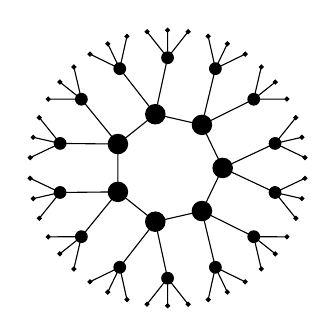
\begin{tikzpicture}[scale=0.7]
        \def\crater{7}
        \foreach \i in {1,...,\crater} {
          \draw[fill] (360/\crater*\i:1cm) circle (5pt);
          \draw (360/\crater*\i : 1cm) -- (360/\crater*\i+360/\crater : 1cm);
          \foreach \j in {-1,1} {
            \draw[fill] (360/\crater*\i : 1cm) -- (360/\crater*\i + \j*360/\crater/4 : 2cm) circle (3pt);
            \foreach \k in {-1,0,1} {
              \draw[fill] (360/\crater*\i + \j*360/\crater/4 : 2cm) --
              (360/\crater*\i + + \j*360/\crater/4 + \k*360/\crater/6 : 2.5cm) circle (1pt);
            }
          }
        }
      \end{tikzpicture}
    \end{column}
  \end{columns}
\end{frame}

%%

\begin{frame}{Volcanology}
  \centering
  \begin{columns}
    \begin{column}{0.35\textwidth}
      \uncover<2->{Height $= v_\ell([\O_K:\Z[\pi]])$.}
      
      \bigskip
      
      \uncover<3->{\alert{How large is the crater?}}
    \end{column}
    \begin{column}{0.65\textwidth}
      \centering
      \begin{tikzpicture}[scale=0.9]
        \begin{scope}
          \def\crater{7}
          \foreach \i in {1,...,\crater} {
            \draw[fill] (360/\crater*\i:1cm) circle (5pt);
            \draw (360/\crater*\i : 1cm) -- (360/\crater*\i+360/\crater : 1cm);
            \foreach \j in {-1,1} {
              \draw[fill] (360/\crater*\i : 1cm) -- (360/\crater*\i + \j*360/\crater/4 : 2cm) circle (3pt);
              \foreach \k in {-1,0,1} {
                \draw[fill] (360/\crater*\i + \j*360/\crater/4 : 2cm) --
                (360/\crater*\i + + \j*360/\crater/4 + \k*360/\crater/6 : 2.5cm) circle (1pt);
              }
            }
          }
        \end{scope}
        \begin{scope}[xshift=4cm]
          \node at (0,2) {$\End(E)$};
          \draw[fill] (0,1) circle(5pt) node[xshift=0.7cm]{$\O_K$} -- 
          (0,0) circle(3pt) --
          (0,-1) circle(1pt) node[xshift=0.7cm]{$\Z[\pi]$};
        \end{scope}
      \end{tikzpicture}
    \end{column}  
  \end{columns}
  
  \bigskip
  
  \begin{tabular}{c | c | c c c}
    && \textbf{Horizontal} & \textbf{Ascending} & \textbf{Descending}\\
    \hline
    $\ell\nmid[\O_K:\O]]$ & $\ell\nmid[\O:\Z[\pi]]$ &$1+\left(\frac{D_K}{\ell}\right)$& &\\
    $\ell\nmid[\O_K:\O]]$ & $\ell\mid[\O:\Z[\pi]]$ &$1+\left(\frac{D_K}{\ell}\right)$& &$\ell-\left(\frac{D_K}{\ell}\right)$\\
    $\ell\mid[\O_K:\O]]$ & $\ell\mid[\O:\Z[\pi]]$ &  &$1$&$\ell$\\
    $\ell\mid[\O_K:\O]]$ & $\ell\nmid[\O:\Z[\pi]]$ & &$1$& 
  \end{tabular}
\end{frame}

%%

\begin{frame}{The class group}
  
  Let \emph{$\End(E) = \O \subset \Q(\sqrt{-D})$}. Define

  \begin{itemize}
  \item $\mathcal{I}(\O)$, the group of \emph{invertible fractional ideals},
  \item $\mathcal{P}(\O)$, the group of \emph{principal ideals},
  \end{itemize}
  
  \begin{block}{The class group}
    The \emph{class group} of $\O$ is
    \[\Cl(\O) = \mathcal{I}(\O)/\mathcal{P}(O).\]
  \end{block}

  \begin{itemize}
  \item It is a \emph{finite abelian} group.
  \item Its order \emph{$h(\O)$} is called the \emph{class number} of
    $\O$.
  \item It arises as the Galois group of an abelian extension of
    $\Q(\sqrt{-D})$.
  \end{itemize}
\end{frame}

%%

\begin{frame}
  \frametitle{Complex multiplication}
  
  \begin{block}{The $\a$-torsion}
    \begin{itemize}
    \item Let \emph{$\a\subset\O$} be an (integral invertible) ideal of
      $\O$;
    \item Let \emph{$E[\a]$} be the subgroup of $E$ annihilated by
      $\a$:
      \[E[\a] = \{P\in E \;|\; \alpha(P) = 0 \text{ for all } \alpha\in\a\};\]
    \item Let \emph{$\phi:E\to E_\a$}, where $E_\a=E/E[\a]$.
    \end{itemize}
    Then $\End(E_\a) = \O$ (i.e., $\phi$ is \emph{horizontal}).
  \end{block}


  \begin{theorem}[Complex multiplication]
    The action on the set of elliptic curves with complex
    multiplication by $\O$ defined by \emph{$\a\ast j(E) = j(E_\a)$}
    factors through $\Cl(\O)$, is faithful and transitive.
  \end{theorem}

  \begin{corollary}
    If $E$ is on the crater of an $\ell$ volcano, the crater contains
    $h(\End(E))$ curves.
  \end{corollary}
\end{frame}

%%

\begin{frame}{Supersingular graphs}
  \begin{columns}
    \begin{column}{0.6\textwidth}
      \begin{itemize}
      \item Every supersingular curve is defined over \emph{$\F_{p^2}$}.
      \item For every \emph{maximal order type} of the quaternion
        algebra $\Q_{p,\infty}$ there are \emph{$1$ or $2$ curves over
          $\F_{p^2}$} having endomorphism ring isomorphic to it.
      \item There is a \emph{unique isogeny class} of supersingular
        curves over $\bar{\F}_p$ of size \emph{$\sim p/12$}.
      \item Left ideals act on the set of maximal orders like isogenies.
      \item The graph of \emph{$\ell$}-isogenies is
        \emph{$(\ell+1)$}-regular.
      \end{itemize}
    \end{column}
    \begin{column}{0.4\textwidth}
      \centering
      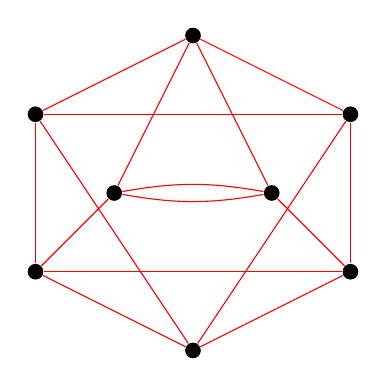
\begin{tikzpicture}
        \begin{scope}[every node/.style={fill,black,circle,inner sep=2pt}]
          \node at (0,0)  (1){};
          \node at (0,4) (20){};
          \node at (2,1)  (16z){};
          \node at (-2,1)  (81z){};
          \node at (-1,2) (77z){};
          \node at (1,2)  (20z){};
          \node at (-2,3)  (85z){};
          \node at (2,3)  (12z){};
        \end{scope}

        \begin{scope}[red]
          \path (1) edge (85z) edge (81z) edge (12z) edge (16z);
          \path (20) edge (85z) edge (77z) edge (20z) edge (12z);
          \path (81z) edge (85z) edge (77z) edge (16z);
          \path (85z) edge (12z);
          \path (12z) edge (16z);
          \path (16z) edge (20z);
          \path (20z) edge[bend right=10] (77z) edge[bend left=10] (77z);
        \end{scope}
      \end{tikzpicture}
      \small
      \emph{Figure:} $3$-isogeny graph on $\F_{97^2}$.
    \end{column}
  \end{columns}
\end{frame}

%%
%% 

\section{Isogeny-based cryptography}
\subsection{Isogeny walks}

%%
%% 

\subsection{Key exchange from ordinary graphs}

%%
%% 

\subsection{Key exchange from supersingular graphs}

% \begin{frame}{The scheme}
  
% \end{frame}

% %%

% \begin{frame}{Attacks}
  
% \end{frame}

% %%

% \begin{frame}{SIKE}
  
% \end{frame}

% %%

% \begin{frame}{Implementation}
  
% \end{frame}

% %%

% \begin{frame}{Side channels}
  
% \end{frame}

% %% 

% \begin{frame}{Key compression? Signatures?}
  
% \end{frame}

%%
%% 

%%

\begin{frame}
  \centering
  \begin{tikzpicture}
    \begin{scope}[xscale=1.2,black!60]
      \def\crater{7}
      \foreach \i in {1,...,\crater} {
        \draw[fill] (360/\crater*\i:3cm) circle (5pt);
        \draw (360/\crater*\i : 3cm) -- (360/\crater*\i+360/\crater : 3cm);
        \foreach \j in {-1,1} {
          \draw[fill] (360/\crater*\i : 3cm) -- (360/\crater*\i + \j*360/\crater/4 : 4cm) circle (3pt);
          \foreach \k in {-1,0,1} {
            \draw[fill] (360/\crater*\i + \j*360/\crater/4 : 4cm) --
            (360/\crater*\i + + \j*360/\crater/4 + \k*360/\crater/6 : 4.5cm) circle (1pt);
          }
        }
      }
    \end{scope}
    
    \draw (0,1) node{\Huge\bf Thank you};
    \draw (0,-0.6) node{\large\url{http://defeo.lu/}};
    \draw (0,-1.3) node{\large
\includegraphics[height=0.9em]{twitter.png}~\href{https://twitter.com/luca_defeo}{@luca\_defeo}};
  \end{tikzpicture}
\end{frame}

%%
%%

% \begin{frame}[allowframebreaks]
%   \frametitle{References}

%   \defbibfilter{books}{\type{book} \or \type{booklet} \or \type{thesis}
%     \or \type{report} \or \type{collection} \or \type{manual}
%     \or \type{periodical} \or \type{proceedings}}
%   \defbibfilter{articles}{\not \(\type{book} \or \type{booklet} \or \type{thesis}
%     \or \type{report} \or \type{collection} \or \type{manual}
%     \or \type{periodical} \or \type{proceedings}\)}

%   \beamertemplatebookbibitems
%   \printbibliography[filter=books]
%   \beamertemplatearticlebibitems
%   \printbibliography[filter=articles]
% \end{frame}

\end{document}


% LocalWords:  Isogeny abelian isogenies hyperelliptic supersingular Frobenius
% LocalWords:  isogenous


